\documentclass[a4paper]{exam}
\usepackage[margin=1in]{geometry}
\usepackage{amsmath, amsfonts}
\usepackage{pythonhighlight}
\usepackage{graphicx} %package to manage images
\graphicspath{ {./images/} }
% \usepackage{tikz}
% \usetikzlibrary{shapes, arrows.meta, positioning}
\usepackage[edges]{forest}

\printanswers
\begin{document}
\begin{center}
{\Large \textbf{Spring 2024}}\vspace{1.0em}\\
{\Large \textbf{CS 412 (Algorithms: Design and Analysis)}}\vspace{1.0em}\\
{\Large \textbf{Weekly Challenge 02: Sorting}}\vspace{1.0em}\\
{\Large Announced: Friday, January 19, 2024.}\\
\vspace{.25em}
{\Large Deadline: Friday, January 26 , 2024 (11:59 pm PKT).}\\ 
\vspace{.3em}
{\Large Total marks: 1.}
\vspace{.5em}\\
\end{center}
Instructions: Submit \textbf{individually} your solution as a PDF with the file name as your $studentID.pdf$; typeset in LaTeX. You must submit your solution on Canvas.

\centerline{\rule{.7\textwidth}{1pt}}

\begin{questions}
\question[1]
A decision tree is a binary tree that represents the comparisons between elements that are performed by a particular sorting algorithm operating on an input of a given size. Control, data movement, and all other aspects of the algorithm are ignored. The leaf nodes represent all possible permutations (arrangements) of the input array. For example, the following is a decision tree of the bubble sort algorithm for $n=3$, where $n$ is the total number of elements in an array.
\begin{center}
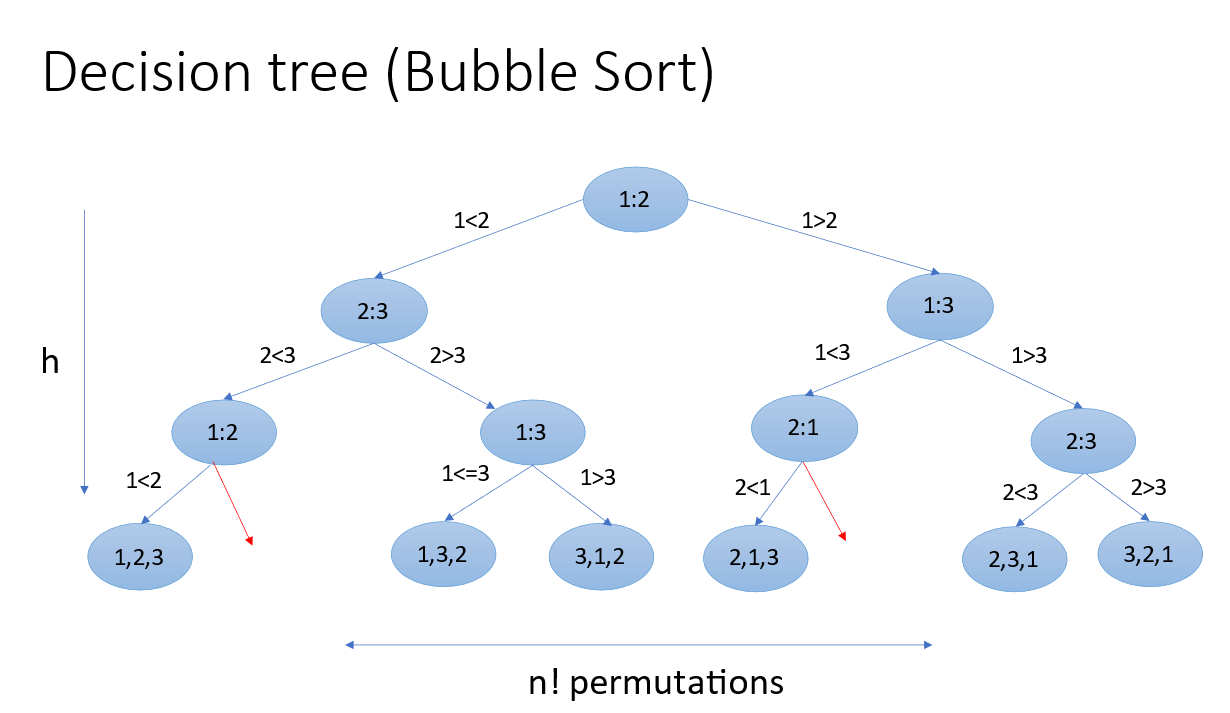
\includegraphics[scale=0.4]{wc02_image.png}    
\end{center}
Take $n=3$ and compare the efficiency of selection sort and insertion sort, in terms of the number of comparisons, with the help of a decision tree when the array is:
\begin{enumerate}
    \item Fully sorted
    \item Fully unsorted
\end{enumerate}

Please draw the decision tree for both algorithms and give your analysis in three to four lines.
\begin{solution}
    % \begin{center}
    %     \begin{tikzpicture}[
    %         node distance=2cm,
    %         block/.style={rectangle, draw, text centered},
    %         decision/.style={diamond, draw, text centered},
    %         arrow/.style={->, >=Stealth}
    %     ]
    %         \node[block] (start) {Start};
    %         \node[decision, below of=start] (compare) {Compare};
    %         \node[block, below left=1.5cm and -1cm of compare] (swap) {Swap};
    %         \node[block, below right=1.5cm and -1cm of compare] (no_swap) {No Swap};
    %         \node[block, below of=no_swap] (end) {End};
    
    %         \draw[arrow] (start) -- (compare);
    %         \draw[arrow] (compare) -- node[above] {Yes} (swap);
    %         \draw[arrow] (compare) -- node[above] {No} (no_swap);
    %         \draw[arrow] (swap) -- (end);
    %         \draw[arrow] (no_swap) -- (end);
    
    %         \node[below=0.5cm of swap] (label_swap) {Swap elements and repeat};
    %         \node[below=0.5cm of no_swap] (label_no_swap) {Move to the next element};
    
    %         \draw (compare) -| ++(3,-0.5) |- (label_swap);
    %         \draw (no_swap) -- (label_no_swap);
    
    %     \end{tikzpicture}
    %     % \captionof{figure}{Insertion Sort Decision Tree (3 elements)}
    %     % \label{fig:decision_tree}
    % \begin{forest}
    %     for tree={
    %       circle,
    %       draw,
    %       s sep=20pt,
    %       text centered,
    %       edge={->, >=stealth},
    %       anchor=center,
    %       tier/.wrap pgfmath arg={tier #1}{level()},
    %     },
    %     [Start
    %       [Compare
    %         [Swap, edge label={node[midway,left] {Yes}}
    %           [End]
    %         ]
    %         [No Swap, edge label={node[midway,right] {No}}
    %           [End]
    %         ]
    %       ]
    %     ]
    %   \end{forest}
    % % \end{center}
    \centering
    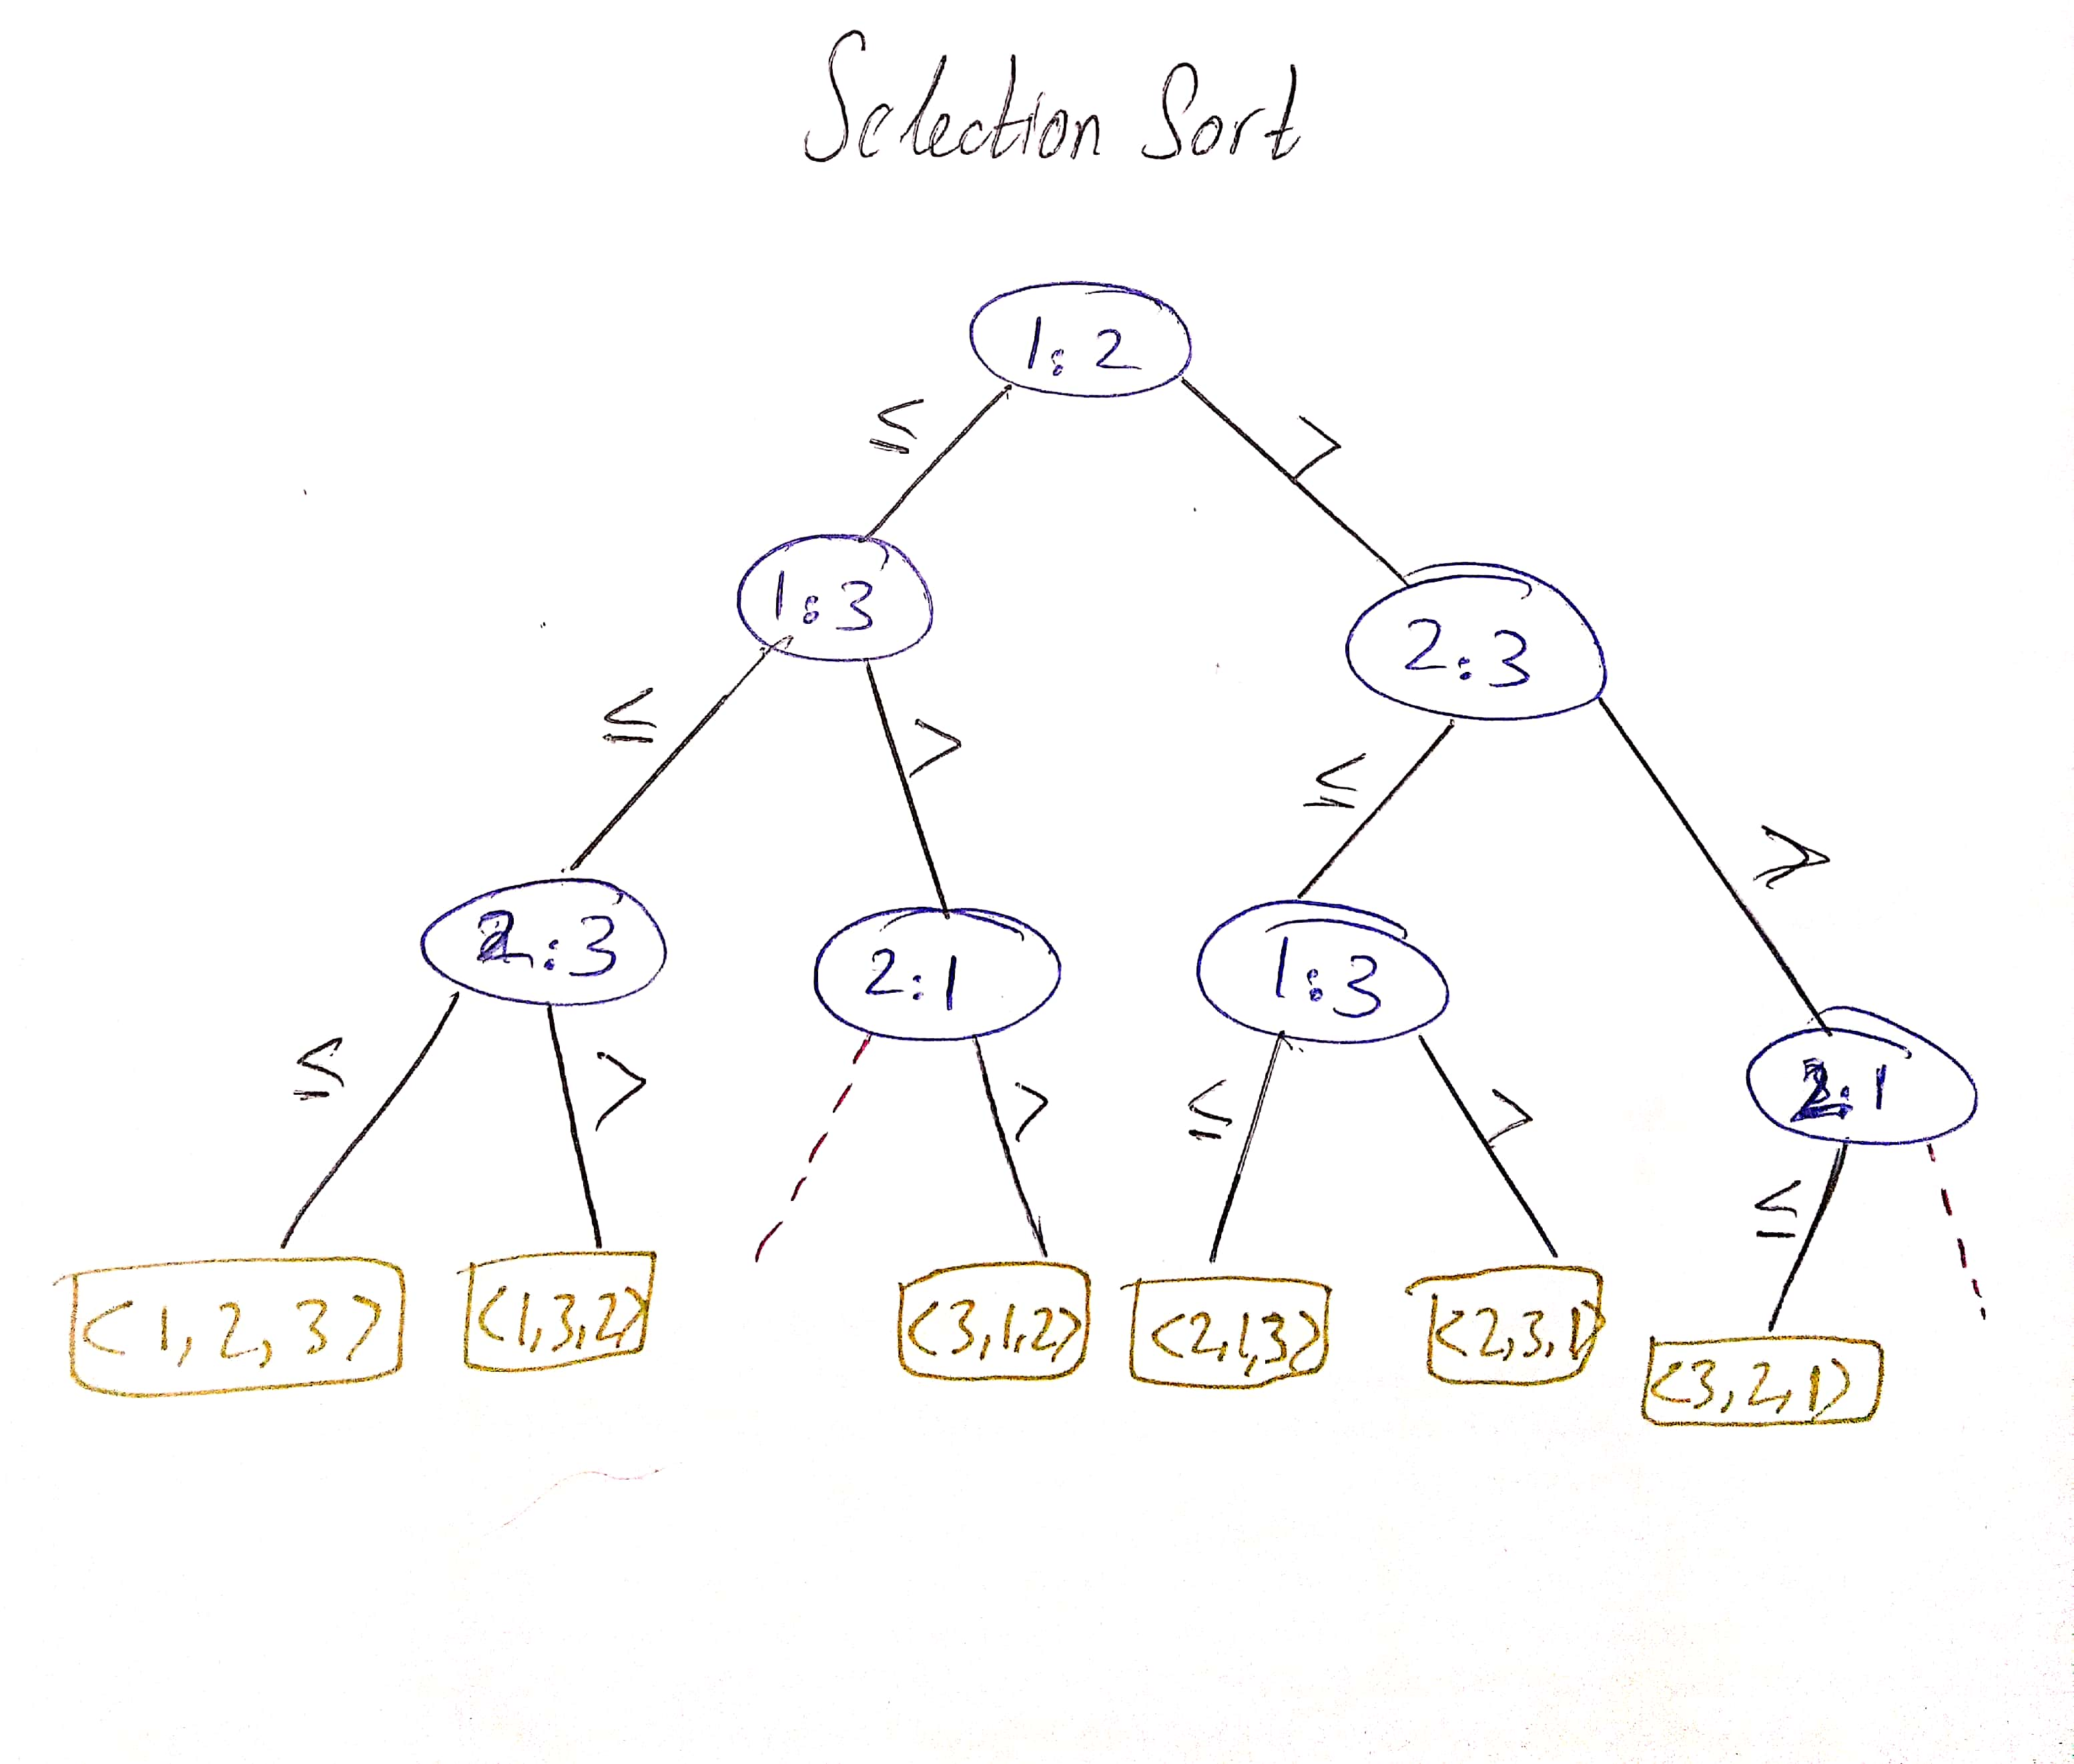
\includegraphics[width=0.8\textwidth]{select.jpeg}
    % \captionof{figure}{Caption for your image}
    % \label{fig:your_label}


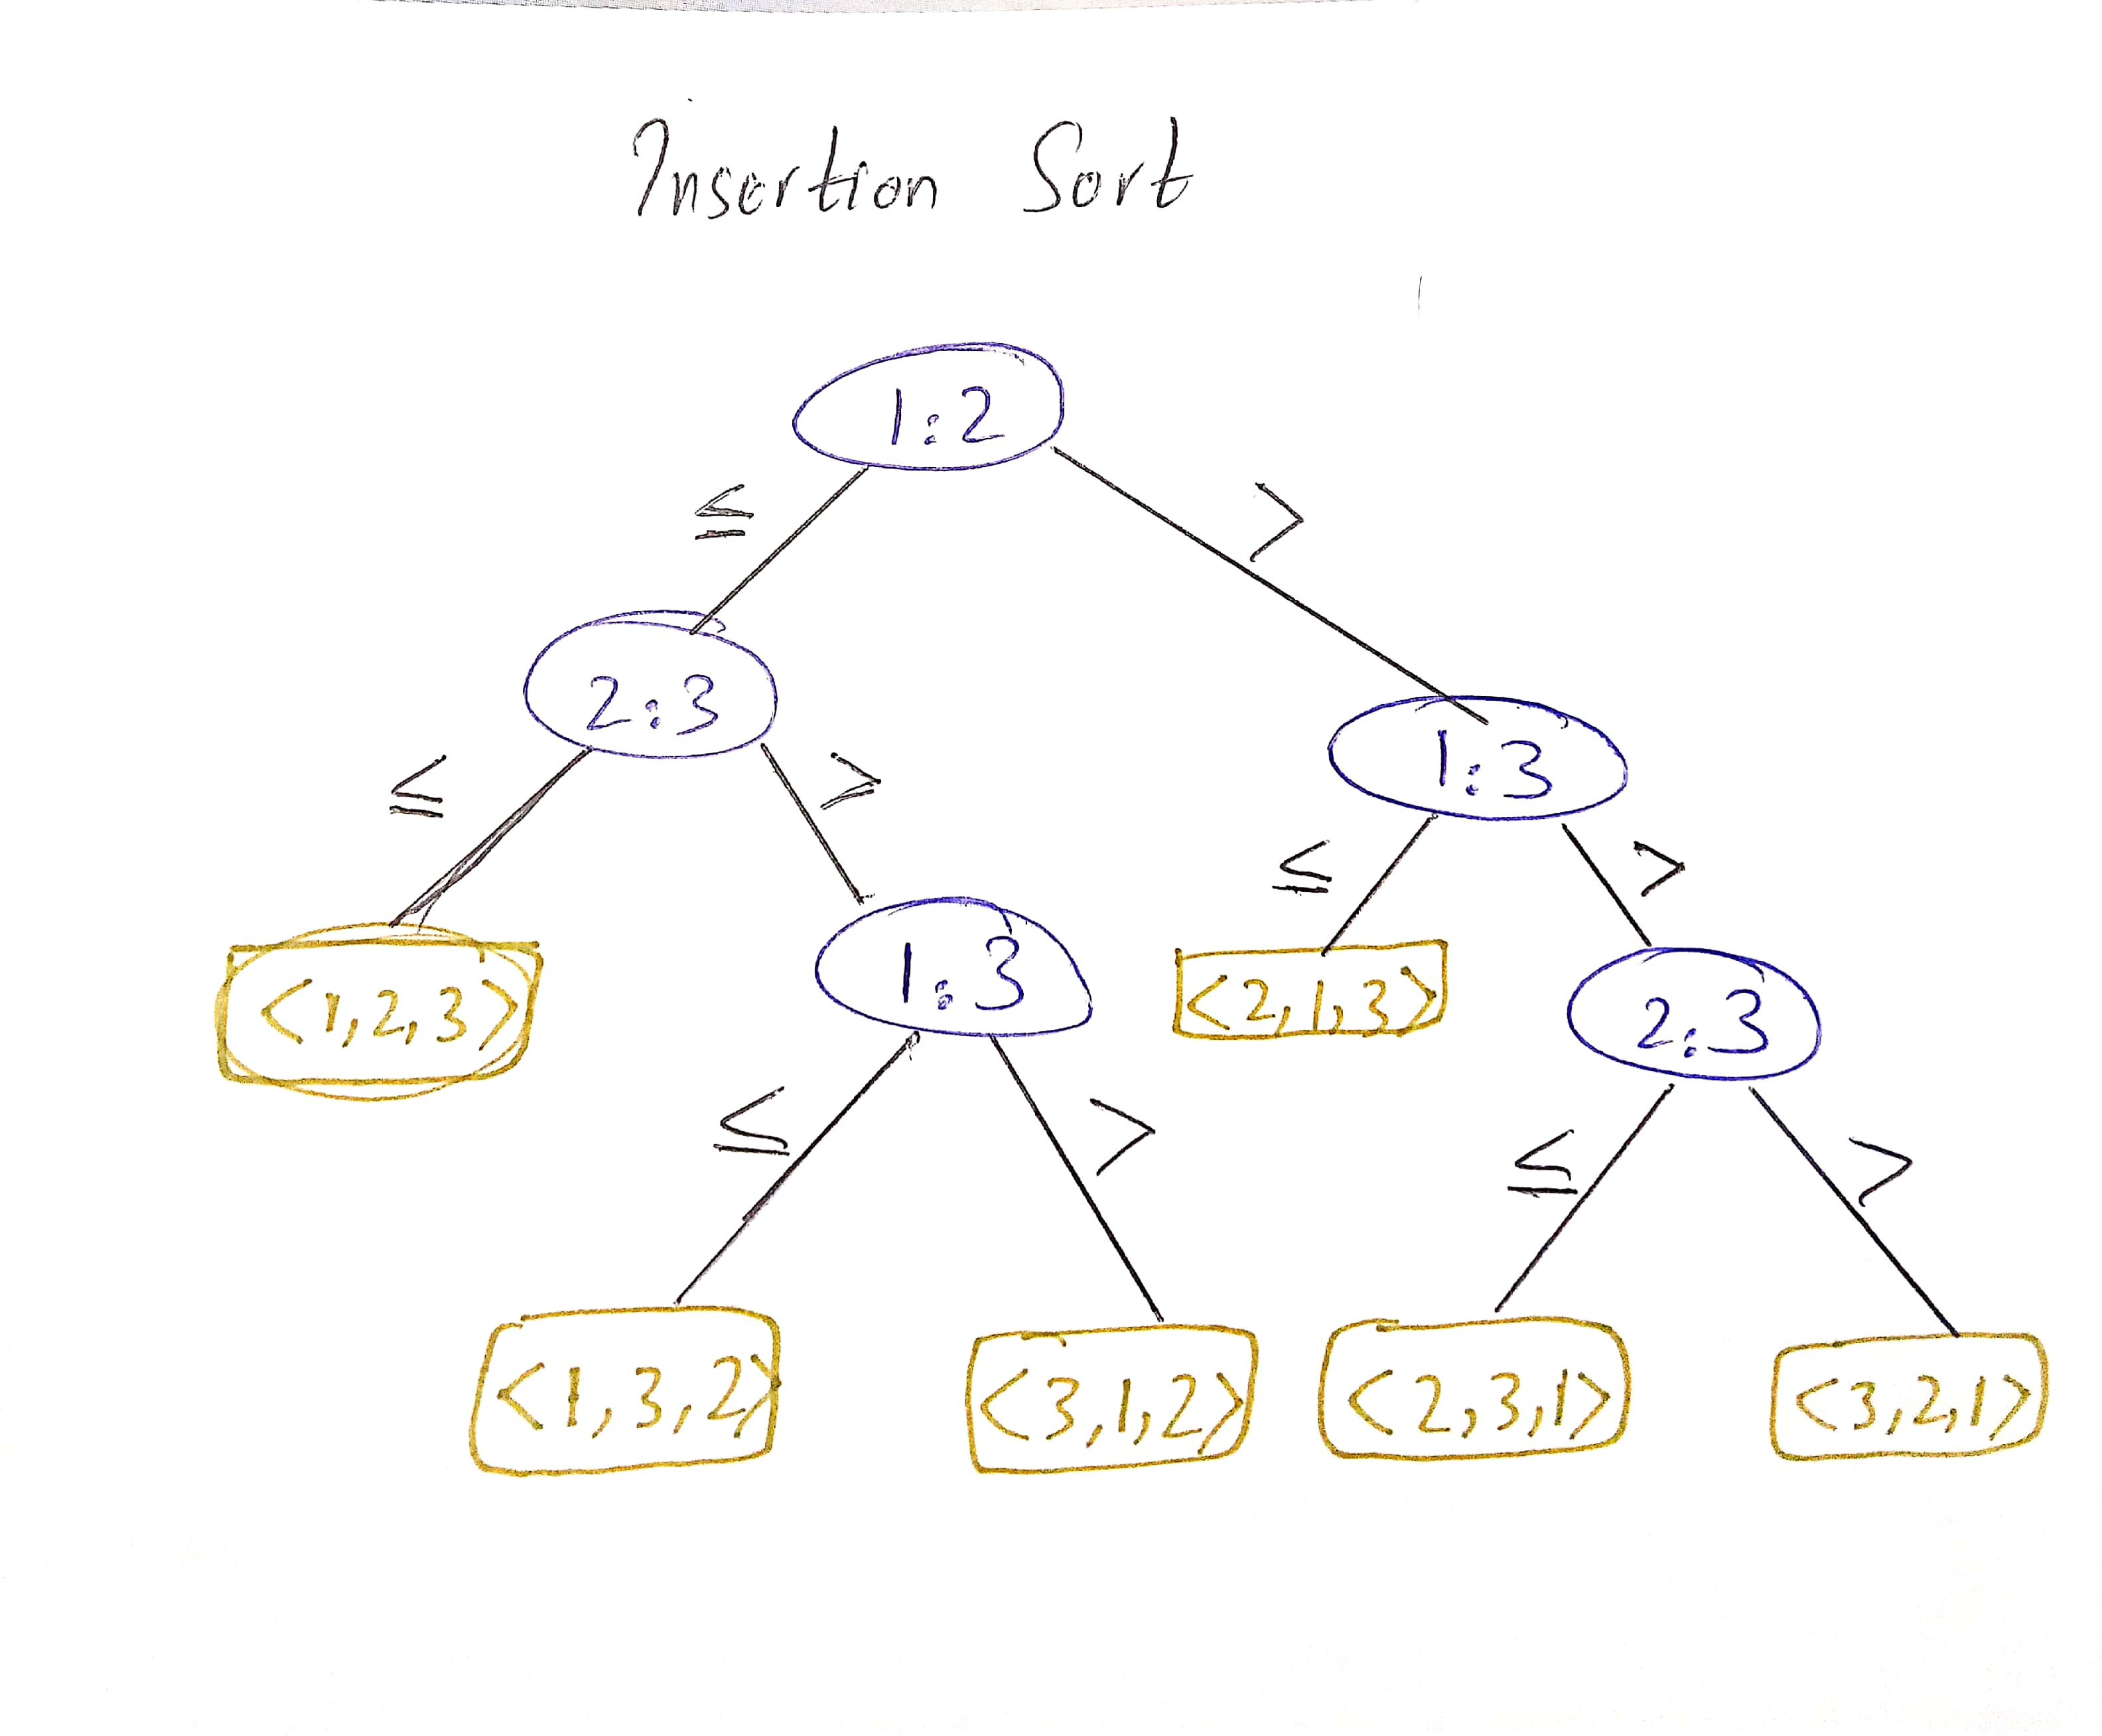
\includegraphics[width=0.8\textwidth]{insert.jpeg}
    % \captionof{figure}{Caption for your image}
    % \label{fig:your_label}

    When we look at it, Selection sort took 3 comparisons in both best and worst cases, while insertion sort took 3 comparisons in the fully unsorted one, while 2 comparisons in the sorted one. This aligns with the idea that the worst and best case complexity of Selection sort is $O(n^2)$ and the worst case complexity of Insertion Sort is $O(n^2)$ and best case is $O(n)$

\end{solution}
\end{questions}

\end{document}
